\section{香港自古以來不就是中國領土嗎?}
回答問題前,總得先解題。這條問題的出現,往往是以反問句而非疑問句的方式,發問者對此已有答案,並以此來質疑別人。「香港自古以來就是中國的領土」這句話常常被拿來支持一些具體的政治立場,例如說香港人不應反抗中央政府的決定,或稱以公投決定香港未來並不可行。

這種質疑有兩個問題。第一,世界不停改變,過去可作參考,卻不足以決定未來。第二,即使香港自古以來是中國領土,考慮到歷朝歷代此地都處於被剝削與犧牲的角色,則不停強調這個「自古以來」的關聯,恐怕對強化香港人的中國認同無甚幫助。

讓我們先把定義釐清。《基本法》序言首句說「香港自古以來就是中國的領土」,不過「香港」這個概念嚴格來說要到英殖時代才開始出現,較準確的說法是香港在內的華南沿岸歷來受中原政權所操控。說到「領土」,中國歷朝歷代的理解和今天的也很不一樣,過去國際邊界不明確和疆土概念模糊,當中「主權」的定義和屬性在中國和歐洲就有節然不同的歷史軌跡;由此出發,古時對「中國」的理解和今天也差距很遠。若要尊重歷史,也該認清楚中國自古以來每個朝代的版圖和上一個朝代的版圖都沒有必然關係,中國的範圍自古以來都在不斷變化。而即使我們認同「香港自古以來就是中國的領土」這句說話,其現實意義仍可爭議:畢竟對於清朝在「不平等條約」下所喪失的領土,當前中國政府並不是每一處都會拿出「自古以來」的說法去宣示權益,中俄邊界就是一例。中國政府會不會或在什麼時候因為某處「自古以來就是中國領土」而選擇引伸或不引伸出一系列的政治立場,從來也相當流動,並不如其政治修辭說得那麼必然。

簡而言之,就算認同「香港自古以來就是中國的領土」這句話,也不能推論出香港於中國現時應有的政治關係,亦不能限制未來中港關係的各種可能。

話雖如此,如果我們把問題反轉過來,以邊緣的角度出發,視之為討論的開端而非終結,則不單可得出節然不同的解讀,更可幫助我們理解香港歷史和社會的複雜性。舉個例,我們可問一問這片現在叫作香港的地方自古以來是在怎樣的意義下演譯其所謂中國領土的地位,中國自古以來是如何理解這個今天稱為香港的地方,而以此構成的關係又如向建立不同時代的中國對香港的理解或誤解。

我們不妨從蜑族人的歷史開始談這個故事。蜑族人是指華南沿岸的水上人,往往以江海為家,居無定所。中國傳統文化以土地為基礎,要到水上生活的往往是因避亂、兵敗、被罰而進入大海,本來就是邊緣地帶的邊緣群體。千年以來,蜑族人一直過著被歧視、被流放、被徵召,然後被鎮壓的命運。蜑族人自漢代以來便被禁止在陸上建屋,不得與陸地居民通婚和出席考試,也不可以購買田土與官位。宋代的時候朝廷曾招引蜑族為海軍,放寬私鹽。後來南宋經濟衰退,重新壟斷造鹽,蜑族反抗,引發了一一九七年的「大嶼山屠殺」,蜑民死傷枕藉。

相對於中央,邊陲地帶往往扮演這種呼之則來,揮之即去的角色,只因其對中央的價值而存在,當地人本身的生活是無須關心的。再說一例:明代和清代都有過大規模的海禁,以保障中原政權,對沿岸邊緣地區則帶來毀滅性的打擊。例如清代的遷界令,當時朝廷為了削弱在台灣的明鄭王朝,要求山東至廣東沿海居民內遷三十至五十里,房屋焚棄不得復界,百姓流離失所。如果說香港「自古以來是中國的一部分」,它作為「一部分」的意義往往就體現於當一只為了中原政權的利益而可隨時犧牲的棋子。硬要反覆強調這個自古以來的關係,從歷史上看帶來傷痛恐怕多於認同。很可惜,中國歷史的書寫對擴張過程中邊緣地帶的反抗和影響,往往會因為其中原視角的基礎而忽視,很多其他邊緣地帶的歷史書寫也面對同樣的問題。

在中原主導的心態下,住在這片後來稱之為香港的地方的人,又會怎樣被書寫呢?首先,他們不是人。從東晉開始,就有所謂「盧亭魚人」的民間傳說。盧亭是什麼?牠是一種半人半魚的生物,《嶺南叢述》當中聲稱「似人非人,獸形鳩舌,椎髻裸體,出沒波濤,能伏水三四日不死」,基本上就是怪物。在現代化前的中國出現這種民間傳說並不奇怪,但也多少反映了香港一帶相對中原來說的蠻荒邊緣位置,最起碼是個神秘莫測的地方,可算是第一代中國大陸對香港的誤解。相對於今天說香港人歧視中國大陸,中原對邊緣的歧視歷史要久遠得多。顛覆一點想,香港人原來是怪物的後裔。近年香港本土思潮興起,盧亭的傳說也再次流行起來,可說成是「你把我看成異類,我卻樂得被確定與你不同」的時空穿越反諷。有劇場作品甚至以盧亭為題,把魚頭人身的錯置體驗在今天重現人前。

\begin{figure}[htbp]
    \centering
    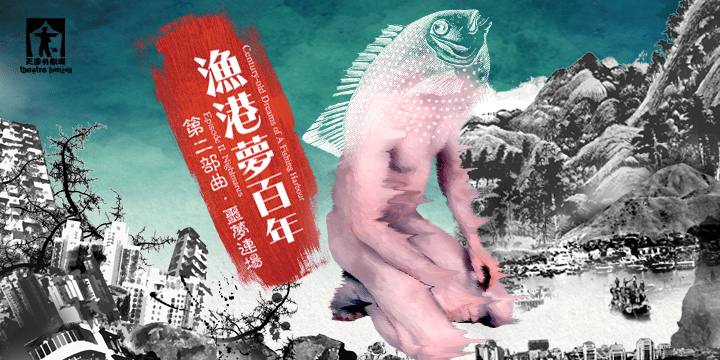
\includegraphics[width=0.7\textwidth]{c01/loting.png}

    % width=3cm[缩放因子], height=8 cm[缩放因子] scale=0.4[缩放因子]
    \caption{《漁港夢百年》第二部曲《噩夢連場》海報} 
\end{figure}

中原對邊陲的輕視歷久不衰,即使在香港被英國佔領後仍可找到這樣的說法。早期英治香港的華文描述,以清朝思想家王韜所寫的為經典。王韜生於蘇州,曾在上海為傳教士工作,還受洗成為基督徒,表面看起來應算是十分思想開明。到了一八六零年,他捲入了太平天國的戰爭,輾轉來到香港避難,是最早在香港長期居留的南來文化人。他剛到埗時對香港的印象並不好,書信中稱「至香一隅,蕞爾絕島」、「竄跡至港,萬非得已」,只是迫於無奈才逃亡至此。提到食物和天氣,他還說「腥聞撲鼻」,和「飛蟲細蚋經冬猶不死」,簡而言之就是個鬼地方。在他眼中,香港就是一個「化外之地」,而且在英殖下還受「化外之民」所統治,不能如歷史文化源遠流長的中原相比。在他早期的寫作中,明顯流露出傳統的華夷觀念,對在香港所見的一切心存敵視。

不過王韜的這些想法卻因他在香港長久生活,和一次長達兩年的歐遊之後有根本改變。他認為中國要全面向西方學習,而香港這個地處邊緣的地方,恰恰成為他能夠發表激進言論的地方。他在香港創辦華文報章,而且每天刊登政論,開風起之先。

在王韜之後,還有很多來自中國大陸的思想家和政治家在香港發表他們對中國時政的看法。香港自開埠以來,好像就不停在辦演一個顛覆者的角色,為中國示範不同的可能。在這兒要總括香港和晚清維新和革命的關係不太可能,只簡單介紹兩個例子。第一位是康有為,他對香港的描述是這樣的:

\begin{displayquote}
    「薄游香港,覽西人宮室之瑰麗,道路之整潔,巡捕之嚴密,乃始知西人治國有法度,不得以古舊之夷狄視之。」(《康南海自編年譜》)
\end{displayquote}

康有為外,當然不能不提在香港學習和成長的孫中山。他說過不少和香港相關的事情,其中以這一段特別聞名:

\begin{displayquote}
    「即從前人人問我,你在何處及如個得到革命思想?吾今直言答之:革命思想,系從香港得來。回憶卅年前,在香港讀書,功課完學,每出外遊行,見得本港衛生與風俗,無一不好,比諸我敝邑香山,大不相同。(……)由此想到香港地方與內地之比較,因香港地方開埠不過七、八十年,而內地已數千年,何以香港歸英國掌管即佈置得如何妥當?」(1923年2月孫中山在香港大學演講)
\end{displayquote}

這些說法嚴格來說也是中國大陸對香港的誤解,當時香港社會也有諸多問題,只是被康有為、孫中山以及一眾文人隱去不提。他們對香港的描述有兩點基本相通。第一,他們重視的不是「香港自古以來就是中國領土」而強調香港和中國大陸的分別,特別是英治之下把本來是中國地方的香港管理得井條有序。第二,他們談論香港的目的並非基於對香港特別有感情,而是要借香港來討論他們對中國政治的立場。香港在這兩段話中的功能是做例子,是他們說故事的工具而非故事的主體。

這點可以說是各種中國大陸對香港誤解的根本原由。把康有為和孫中山的說法,和傳統華夷觀念的說法作比較,當然可看到很明顯的分別,起碼香港的地位被大幅提高;但與此同時,香港之所以會出現的理由卻一脈相承:中國是主題,香港是特例。

當然,個人經歷的不同,往往對描述的內容有決定性的影響。胡適在一九三五年曾經寫過香港,內容是他來訪香港演講見聞,還特別提到大埔的風景美麗。不過說到對香港的具體關懷,則還是回到英治下的中文教育,還提倡香港的小學要徹底改用國語課本。比他早數年來香港的魯迅即沒那麼幸運 ,把前來香港視為「畏途」,因為他在來港的船上被港方關員(他稱為「掛英旗的同胞」)索取賄賂和受不禮貌對待,更把他的書和行李打翻。魯迅繪形繪聲的描述他被關員留難的經歷,不過他到最後仍然不忘其中國視角,說「高等華人」和「一伙作倀的奴氣同胞」,正是中國許多地方的寫照。

從歷史看,如果說「香港自古以來就是中國的領土」,則香港所屬的華南沿岸從來都是以一個邊緣地區的位置和一個與中原文化相對應的地位來被理解,並因而產生諸多誤解。香港所處的邊緣地位,正是此地「自古以來」的核心問題。對香港的理解或誤解,背後是一套中央與邊陲的互動。

人類文明中選擇性描述和遺忘可謂彼彼皆是,中國大陸對香港的描述只是一例。因出發點不同而產生誤解,本屬正常。正如香港人認識中國大陸,也往往會因為香港本身的歷史、環境、社會以及世界觀而變得有選擇性,甚至有所偏差。然而當兩者涉及權力關係,而擁有權力的一方基於誤解來處理這關係,作出違反對方認知的決定時,就可帶來嚴重的矛盾和反彈。

看今天的中港矛盾,不難發現其中一個主因就來自中華人民共和國對香港歷史的官方解讀,和香港人對自己的解讀之間有嚴重落差。而當中國政府基於這些認識為香港作決定時,就往往會在香港社會帶來極大反響。對「香港自古以來就是中國的領土」這句話的不同理解,只是香港眾多同類問題之一。


伸延閱讀:
潘毅、余麗文(2003):〈導言:寫在書寫之前〉,

潘毅、余麗文編:《書寫城市:香港的身分與文化》,香港:牛津大學出版社,頁 xiii-xx。

盧瑋鑾編(1983):《香港的憂鬱:文人筆下的香港 (一九二五—一九四一)》,香港:華風書局。

孔誥烽(1997):〈千年的壓迫、千年的抵抗:殖民主義前後的大澳蛋族〉,

羅永生編:《誰的城市:戰後香港的公民文化與政治論述》,香港:牛津大學出版社,頁 113-140。